\chapter{An interactive walk through the tool}
\label{interactions}

This chapter walks through some interactions with the tool. Design and implementation of the tool was discussed in chapter \ref{chap:overview} and \ref{chap:algorithms}. Instances of the tool's response to specific input and user stimuli are shown here.

A sample text file containing a CFG is passed as an argument to the tool. The grammar is shown in figure \ref{fig:grammar}. This grammar used as a basis for generating questions. Upon receiving this grammar as input, the tool displays a menu to the user asking her to choose the domain for which problems are to be asked. This is shown in figure \ref{fig:main-menu}. Based on this choice, a primary problem is generated for one of the values in the data structure generated during preprocessing. These values are basically the non-terminals in the grammar. This primary problem is shown in figure \ref{fig:primary-ques}. As shown in the image, the question was asked about the first set of a non-terminal in the grammar. The user fills some options as the solution to the problem. As the answer is correct for the above question, then next primary question is generated for the next non-terminal. This is shown in figure \ref{fig:primary-correct}.

However, if the answer is wrong then the tool generates hint questions. In this case, the user enters a set of options (id, *) out of which there is an incorrect option (according to grammar, First[F] is \{id, (\}). Here the tool generates a hint question of type 1 (H1), for each wrong option selected. Since there is one such wrong option (*), the tool generates a hint question (H1) for it. Figure \ref{fig:hint-h1} shows this scenario. 

Now, if the answer to this question is wrong, then system generates this same question repeatedly, until it gets the right answer. This is shown in figure \ref{fig:hint-repeat}. If the user now answers this question correctly, the tool generates a hint question of type 2 for the correct option left unmarked. Figure \ref{fig:hint-h1-h2} shows this scenario.

\begin{figure}
\centering
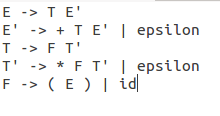
\includegraphics[width=0.8\textwidth]{grammar.png}
\caption{A Context Free Grammar given as input}
\label{fig:grammar}
\end{figure}

\begin{figure}
\centering
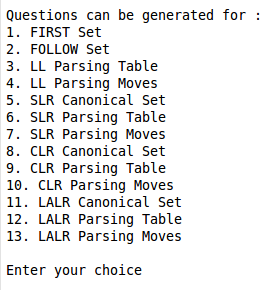
\includegraphics[width=0.8\textwidth]{menu.png}
\caption{A main menu showing the possible domains for which problems can be generated}
\label{fig:main-menu}
\end{figure}

\begin{figure}
\centering
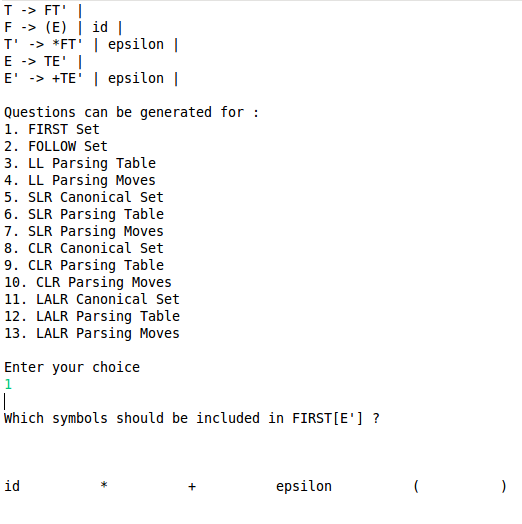
\includegraphics[width=0.8\textwidth]{PrimaryQuestion.png}
\caption{Primary question asked by the tool}
\label{fig:primary-ques}
\end{figure}

\begin{figure}
\centering
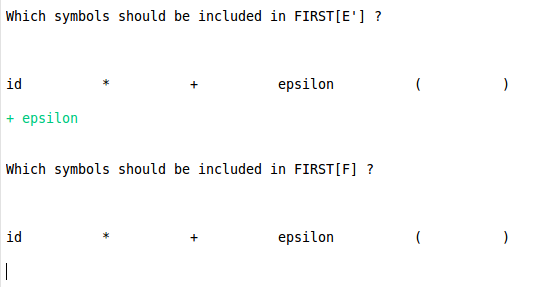
\includegraphics[width=0.8\textwidth]{NextPrimaryQ.png}
\caption{Tool's response to a correct answer by the user}
\label{fig:primary-correct}
\end{figure}

\begin{figure}
\centering
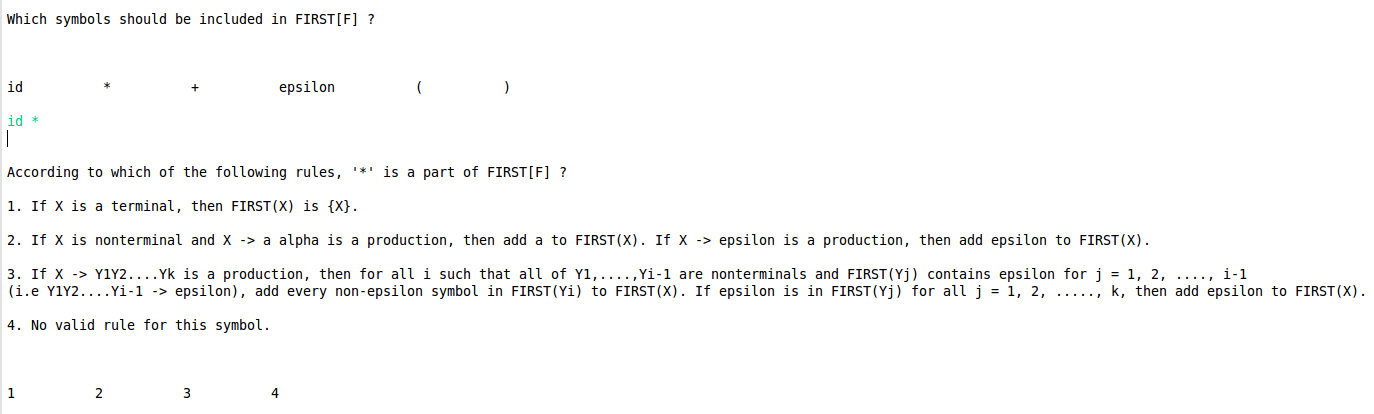
\includegraphics[width=0.8\textwidth]{Type1Incorrect.png}
\caption{Hint question of type 1 generated for incorrect option}
\label{fig:hint-h1}
\end{figure}

\begin{figure}
\centering
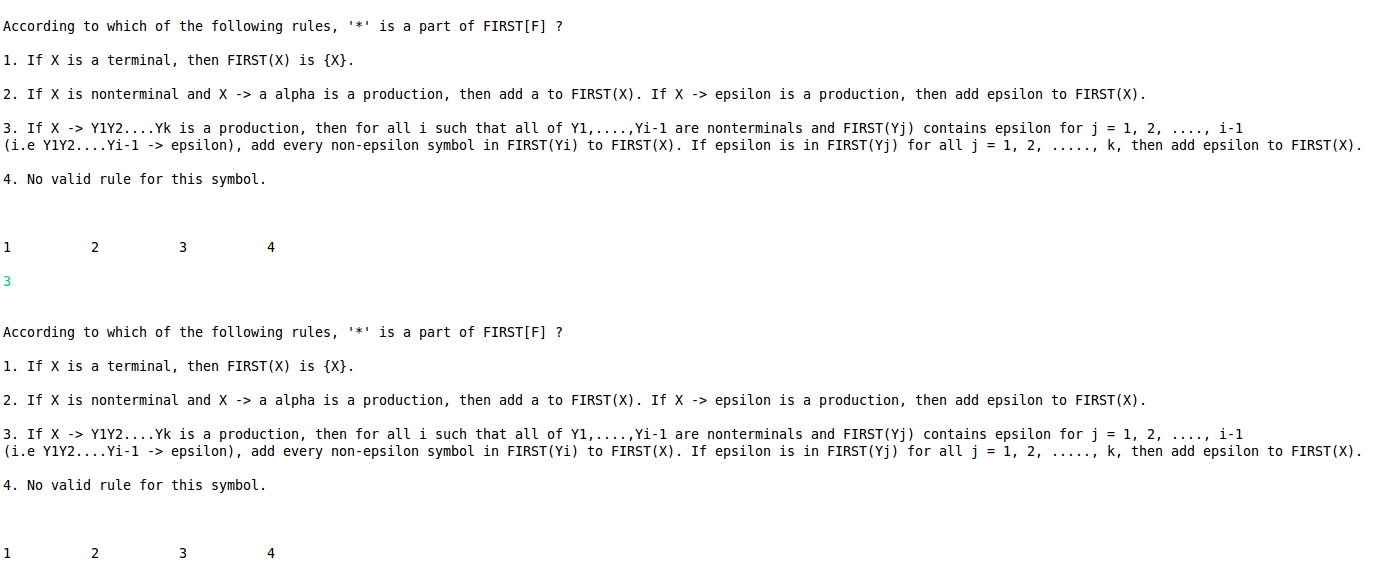
\includegraphics[width=0.8\textwidth]{Type1IncorrectRepeat.png}
\caption{Repetition of hint question due to incorrect attempt}
\label{fig:hint-repeat}
\end{figure}

\begin{figure}
\centering
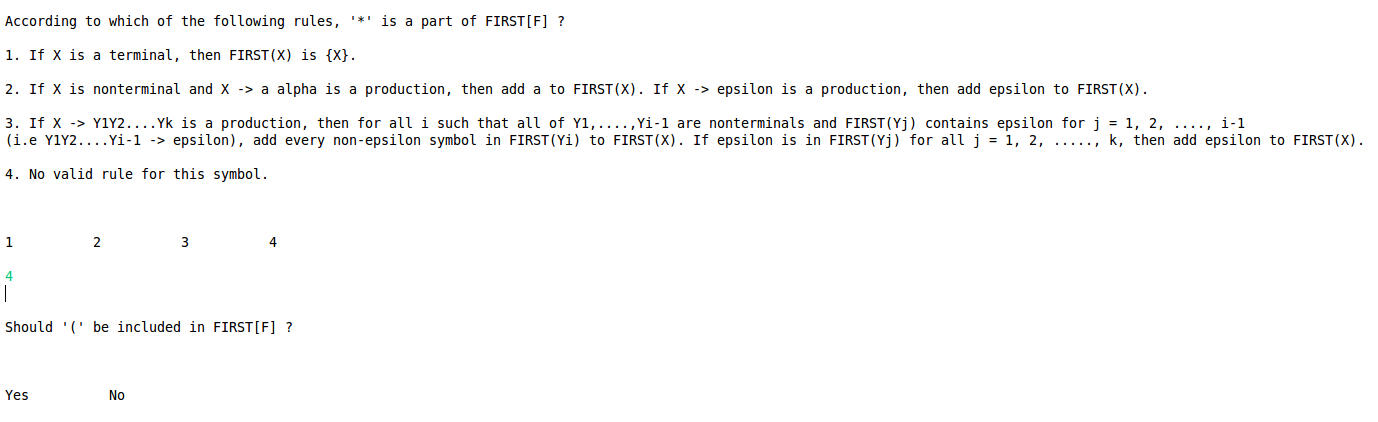
\includegraphics[width=0.8\textwidth]{Type2Correct.png}
\caption{H2 generated when user answers correctly}
\label{fig:hint-h1-h2}
\end{figure}

Again, if the user marks wrong option, then it generates the same question until she choose the right option.

\begin{figure}
\centering
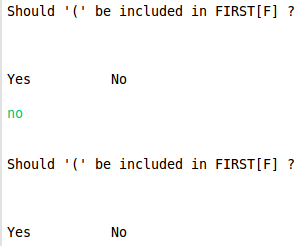
\includegraphics[width=0.8\textwidth]{Type2CorrectRepeat.png}
%\caption{Tree after applying Dijkstra Algorithm second time}
%\label{fig:Dijkstra Tree 2}
\end{figure}

After receiving the correct answer for previous question, the tool generates hint question of type 1 for this correct option. This question asks about the rule by which this value must be a part of correct answer for the primary question.

\begin{figure}
\centering
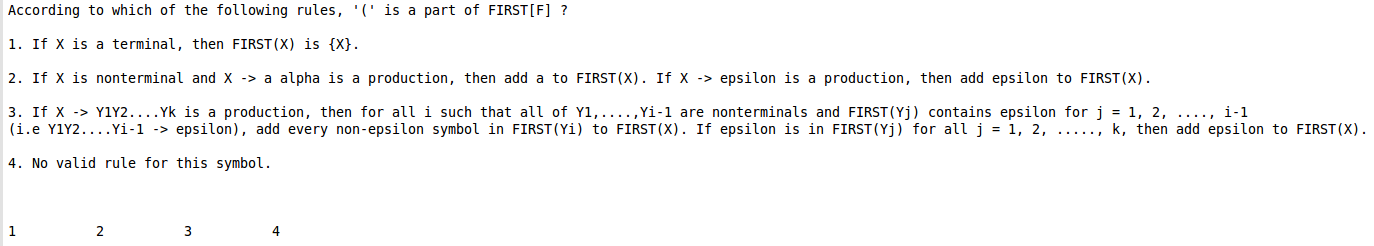
\includegraphics[width=0.8\textwidth]{Type1Correct.png}
%\caption{Tree after applying Dijkstra Algorithm second time}
%\label{fig:Dijkstra Tree 2}
\end{figure}

Again, if the rule marked is wrong, then the tool repeats the question, until correct rule is received.

\begin{figure}
\centering
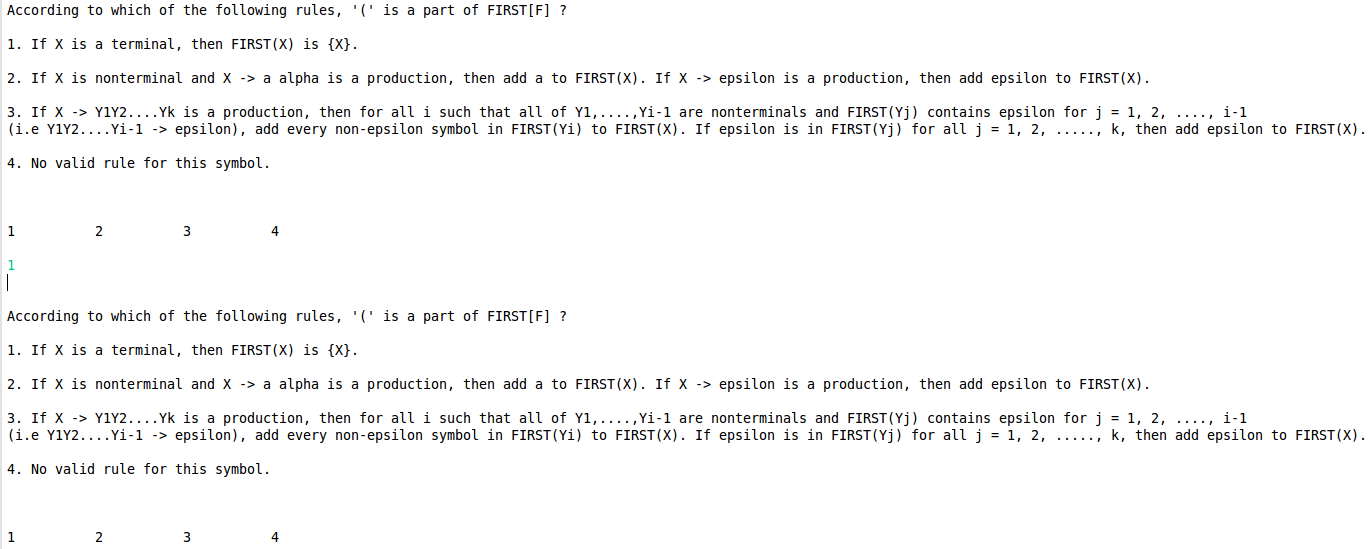
\includegraphics[width=0.8\textwidth]{Type1CorrectRepeat.png}
%\caption{Tree after applying Dijkstra Algorithm second time}
%\label{fig:Dijkstra Tree 2}
\end{figure}

On getting right answer to the above hint question, the tool again generates the same primary question, to check whether the user understands the solution for the question well or not.

\begin{figure}
\centering
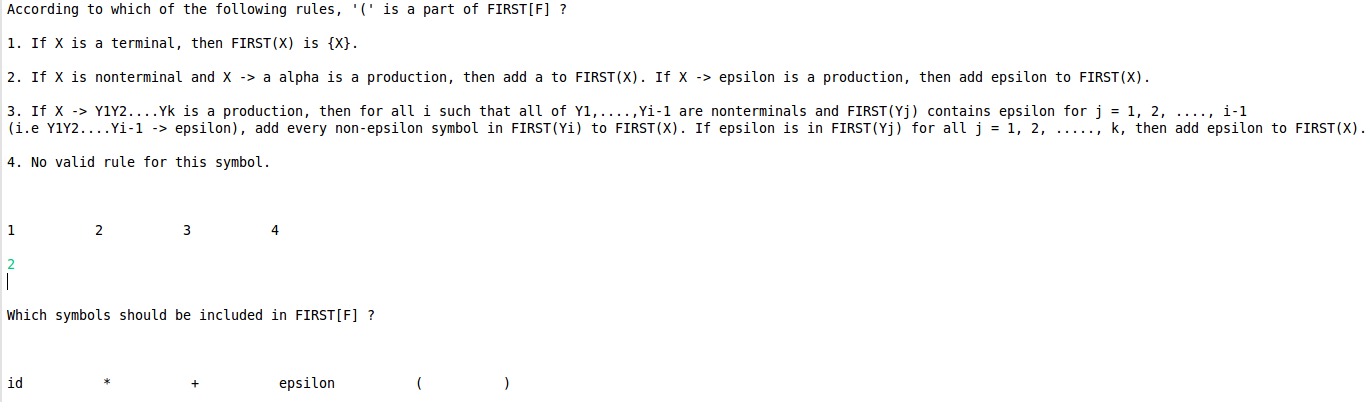
\includegraphics[width=0.8\textwidth]{PrimaryQRepeat.png}
%\caption{Tree after applying Dijkstra Algorithm second time}
%\label{fig:Dijkstra Tree 2}
\end{figure}

If this time, the user gives the right answer, then next primary question is generated. Otherwise, the process repeats, until the tool obtains the right answer of the primary question from the user.

\begin{figure}
\centering
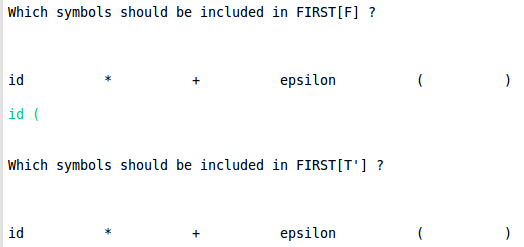
\includegraphics[width=0.8\textwidth]{NewPrimaryQ.png}
%\caption{Tree after applying Dijkstra Algorithm second time}
%\label{fig:Dijkstra Tree 2}
\end{figure}

The process is repeated for the rest of the values.

\section{Level 2 of LL Parsing Table}
The primary question, for this level of LL Parsing Table, remains same as in level 1 of LL Parsing Table. 

\begin{figure}
\centering
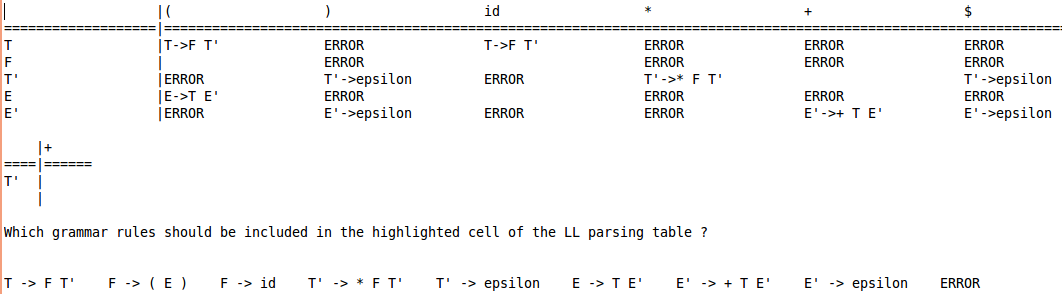
\includegraphics[width=0.8\textwidth]{llTableL2Primary.png}
%\caption{Tree after applying Dijkstra Algorithm second time}
%\label{fig:Dijkstra Tree 2}
\end{figure}

Firstly, it asks primary questions for all the values.
\begin{figure}
\centering
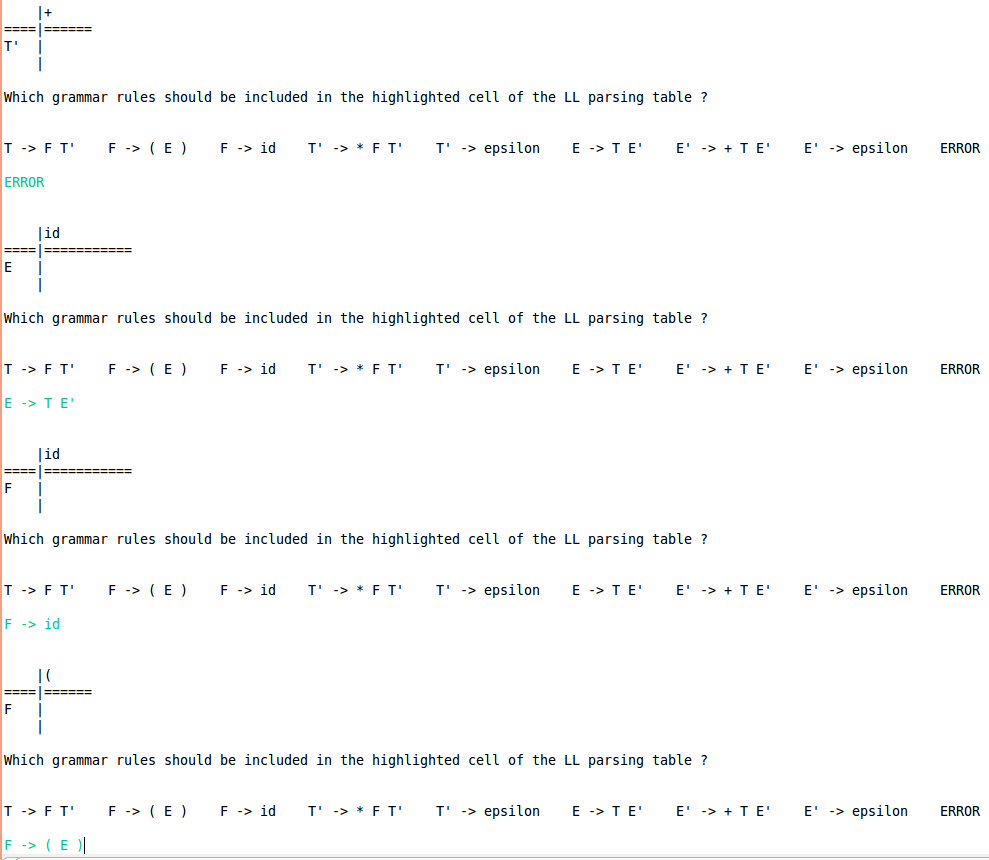
\includegraphics[width=0.8\textwidth]{LLlevel2Primary.png}
%\caption{Tree after applying Dijkstra Algorithm second time}
%\label{fig:Dijkstra Tree 2}
\end{figure}

Then it generates hint questions for all the cells in which user has filled wrong entry. But there is a change in the hint questions. For hints, the tool automatically calculates an input string for the cell, in which user has filled wrong entry. The tool parses this input string, using the LL Parsing table filled by the user. Then in the hint question, the tool shows the moves of the parser on this input string and ask the user to fill the cell again.
\begin{figure}
\centering
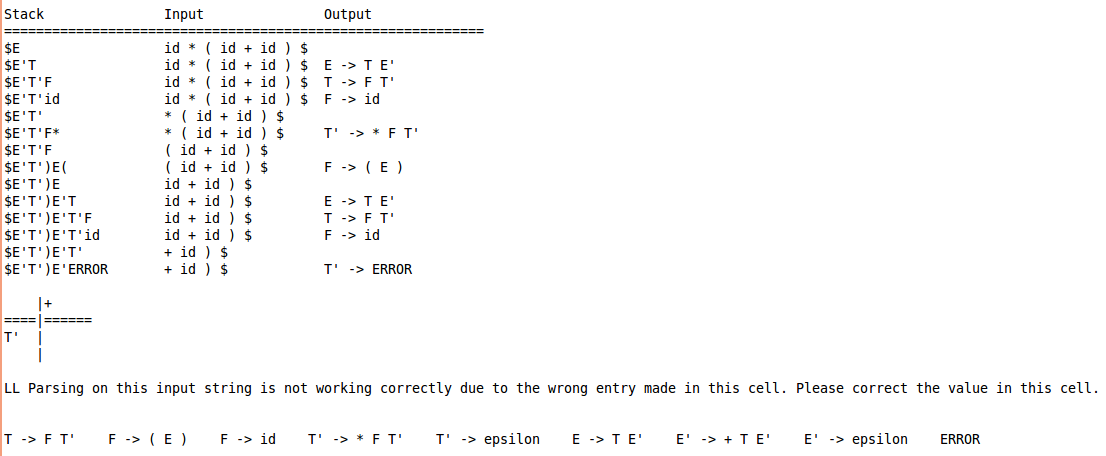
\includegraphics[width=0.8\textwidth]{Level2Hint.png}
%\caption{Tree after applying Dijkstra Algorithm second time}
%\label{fig:Dijkstra Tree 2}
\end{figure}

\section{Level 2 of GOTO}
In level 2 of GOTO function, format of primary problem is the reverse of those in level 1.
\begin{figure}
\centering
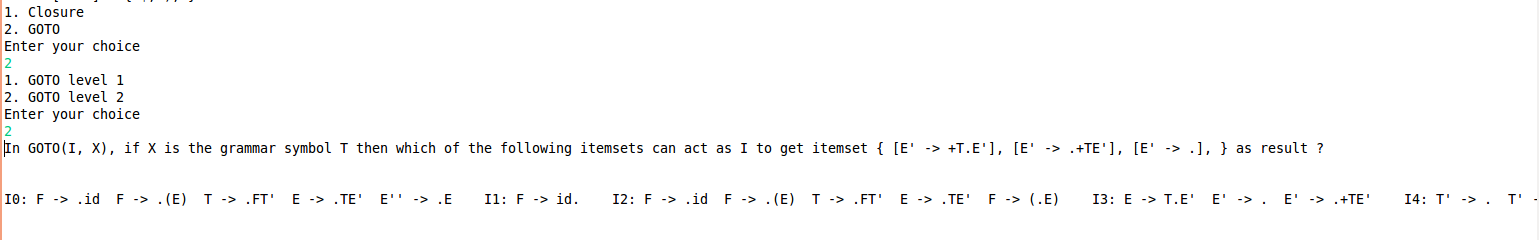
\includegraphics[width=0.8\textwidth]{Level2GOTOPrimary.png}
%\caption{Tree after applying Dijkstra Algorithm second time}
%\label{fig:Dijkstra Tree 2}
\end{figure}

The content of hint questions and their sequence is a little different. Two questions are asked for each wrong option selected and 1 question for each right answer left unmarked in solution. H1 and H3 are of similar type.
H1 for incorrect:
\begin{figure}
\centering
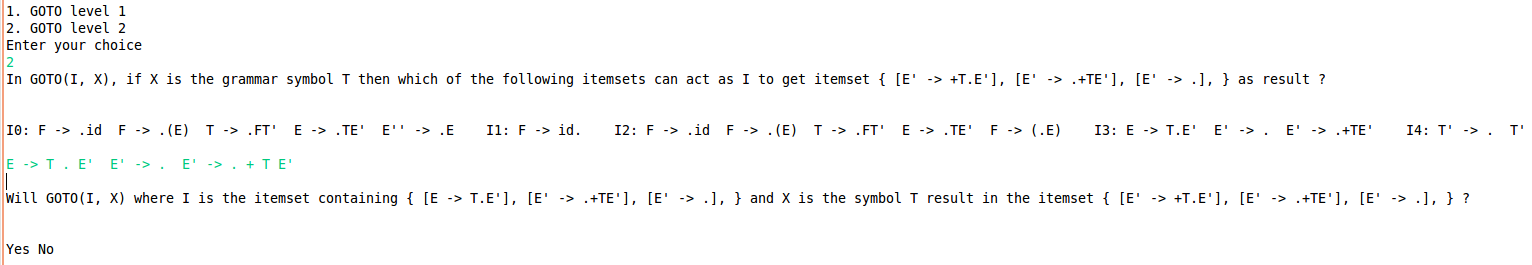
\includegraphics[width=0.8\textwidth]{Level2GotoH1.png}
%\caption{Tree after applying Dijkstra Algorithm second time}
%\label{fig:Dijkstra Tree 2}
\end{figure}

H2 for same incorrect,
\begin{figure}
\centering
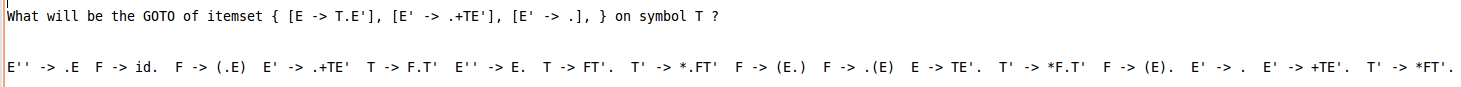
\includegraphics[width=0.8\textwidth]{Level2GotoH2.png}
%\caption{Tree after applying Dijkstra Algorithm second time}
%\label{fig:Dijkstra Tree 2}
\end{figure}

H3 for correct one(or H1 for correct),
\begin{figure}
\centering
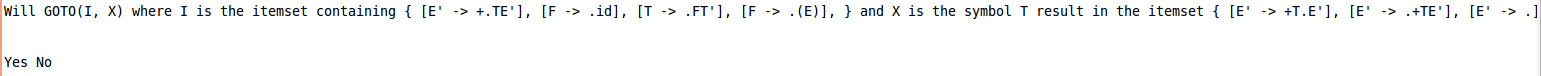
\includegraphics[width=0.8\textwidth]{Level2GotoH3.png}
%\caption{Tree after applying Dijkstra Algorithm second time}
%\label{fig:Dijkstra Tree 2}
\end{figure}